%LaTeX template : http://systbio.org/files/SB_LaTeX_Template_txt_extension.txt
%Author instructions: http://www.oxfordjournals.org/our_journals/sysbio/for_authors/ms_preparation.html


% This version is currently approx 5000 words
%Other versions:
% Science: http://www.sciencemag.org/site/feature/contribinfo/prep/gen_info.xhtml#original_research
        %Research Articles (up to ~4500 words, including references, notes and captions, or ~5 printed pages) are expected to present a major advance. Research Articles include an abstract, an introduction, up to six figures or tables, sections with brief subheadings, and about 40 references. Materials and Methods should usually be included in supplementary materials, which should also include information needed to support the paper's conclusions.
% Nature communications: http://www.nature.com/ncomms/authors/submit.html#Manuscript-text ~5000 words
% PNAS: http://www.pnas.org/site/authors/format.xhtml
% Current Biology: http://www.cell.com/current-biology/authors
        %Articles present conceptual advances of unusual significance regarding a biological question of wide interest. Articles are typically limited to ten journal pages (usually around 5000 words of main text, i.e. all of the text in the manuscript except for the summary, references, and any Supplemental Information text), and there should be no more than seven display items (figures and tables). Additional items and details may be published online as Supplemental Information at the discretion of the editor (please see the Supplemental Information guidelines for more information).
% PLoS Biology: http://journals.plos.org/plosbiology/s/submission-guidelines
% Scientific reports: http://www.nature.com/srep/authors/index.html#initial-submission
        %Articles should be no more than 11 typeset pages in length. As a guide, the main text (not including Abstract, Methods, References and figure legends) should be no more than 4,500 words. The maximum title length is 20 words. The Abstract — which must be no more than 200 words long and contain no references — should serve both as a general introduction to the topic and as a brief, non-technical summary of the main results and their implications. For the main body of the text, there are no explicit requirements for section organization. According to the authors' preference, the text may be organized as best suits the research. As a guideline and in the majority of cases, however, we recommend that you structure your manuscript as follows: Introduction; Results (with subheadings); Discussion (without subheadings);Methods



\documentclass[12pt,letterpaper]{article}
\usepackage{natbib}

%Packages
\usepackage{pdflscape}
\usepackage{fixltx2e}
\usepackage{textcomp}
\usepackage{fullpage}
\usepackage{float}
\usepackage{latexsym}
\usepackage{url}
\usepackage{epsfig}
\usepackage{graphicx}
\usepackage{amssymb}
\usepackage{amsmath}
\usepackage{bm}
\usepackage{array}
\usepackage[version=3]{mhchem}
\usepackage{ifthen}
\usepackage{caption}
\usepackage{hyperref}
\usepackage{amsthm}
\usepackage{amstext}
\usepackage{enumerate}
\usepackage[osf]{mathpazo}
\usepackage{dcolumn}
\usepackage{lineno}
\usepackage{dcolumn}
\newcolumntype{d}[1]{D{.}{.}{#1}}

\pagenumbering{arabic}


%Pagination style and stuff
\linespread{2}
\raggedright
\setlength{\parindent}{0.5in}
\setcounter{secnumdepth}{0} 
\renewcommand{\section}[1]{%
\bigskip
\begin{center}
\begin{Large}
\normalfont\scshape #1
\medskip
\end{Large}
\end{center}}
\renewcommand{\subsection}[1]{%
\bigskip
\begin{center}
\begin{large}
\normalfont\itshape #1
\end{large}
\end{center}}
\renewcommand{\subsubsection}[1]{%
\vspace{2ex}
\noindent
\textit{#1.}---}
\renewcommand{\tableofcontents}{}
%\bibpunct{(}{)}{;}{a}{}{,}

%---------------------------------------------
%
%       START
%
%---------------------------------------------

\begin{document}

%Running head
\begin{flushright}
Version dated: \today
\end{flushright}
\bigskip
\noindent RH: Cretaceous-Palaeogene extinction does not affect mammalian disparity.

\bigskip
\medskip
\begin{center}

\noindent{\Large \bf Cretaceous-Palaeogene extinction does not affect mammalian disparity.} 
% NC: still think this might need some work

\bigskip

\noindent {\normalsize \sc Thomas Guillerme$^1$$^,$$^2$$^*$, and Natalie Cooper$^1$$^,$$^2$$^,$$^3$}\\
\noindent {\small \it 
$^1$School of Natural Sciences, Trinity College Dublin, Dublin 2, Ireland.\\
$^2$Trinity Centre for Biodiversity Research, Trinity College Dublin, Dublin 2, Ireland.\\
$^3$Department of Life Sciences, Natural History Museum, Cromwell Road, London, SW7 5BD, UK.}\\
\end{center}
\medskip
\noindent{*\bf Corresponding author.} \textit{Zoology Building, Trinity College Dublin, Dublin 2, Ireland; E-mail: guillert@tcd.ie; Fax: +353 1 6778094; Tel: +353 1 896 2571.}\\
\vspace{1in}

%Line numbering
\modulolinenumbers[1]
\linenumbers

%---------------------------------------------
%
%       ABSTRACT
%
%---------------------------------------------

\newpage
\begin{abstract}
% NC: As ever I'm ignoring this until we are finished with the rest!
%Massive global extinctions have a turn-over effect on biodiversity. When some large group of taxa suffers from a high rate of extinction, it is expected that niches becomes available for potentially unrelated clades that can undergo an adaptive radiation to fill these vacant niches.
%Therefore, in a context of current global biotic and abiotic changes, resolving this question is crucial to understand the effect of mass extinction events on biodiversity.
%The causes and effects of such events are well understood for marine organisms with a good fossil record (e.g. Ammonoidea and Foraminifera) but the effects remains unclear on some iconic vertebrate groups.

%Typically, placental mammals (eutherians) are shown by some studies to be undergoing an adaptive radiation after the Cretaceous-Palaeogene mass extinction event (K-Pg) by originating shortly before the K-Pg event and displaying high morphological evolutionary rates leading to high diversification during the Palaeogene. However, some other studies have demonstrated that eutherians originates during the Cretaceous and don't display significantly high diversification after the K-Pg event.

%Here we propose a new approach to test if eutherians undergo an adaptive radiation after the K-Pg event. We use trees containing both living and fossil taxa based on all the available data (Total Evidence) and the state-of-the-art method in dating (tip dating) along side with a better proxy for niche occupancy (morphological diversity as opposed to taxonomic diversity) and finer grain analysis through time (introducing a time slicing method).

%Our results shows that mammals don't display significantly changes in morphological disparity that expected under a Brownian motion after the K-Pg boundary. We therefore propose that eutherian mammals don't undergo an adaptive radiation during the Palaeogene.

%Why is our stuff better?
%1-More accurate timing (TEM+tip dating vs. molecular node date or morphological parsimony)
%2-Better proxy for niche occupancy (morphological disparity + diversity vs. species diversity) (but niches concept is shite anyway)
%3-Better measure for disparity (centroid distance vs. Foote's quartet)
%4-Two evolutionary models instead of one for looking at disparity through time (punctuated+constant vs. punctuate)
%5-Systematic time units for looking at disparity through time (slices vs. intervals)

\end{abstract}

\noindent (Keywords: disparity, diversity, punctuated equilibrium, gradualism, time slicing)\\
% NC: Note that keywords are things that aren't in the title of the paper
\vspace{1.5in}

\newpage 

%---------------------------------------------
%
%       INTRODUCTION
%
%---------------------------------------------

\section{Introduction}
% 1§ mass extinctions = bad. Loss of species (e.g. P/T 95%). But what comes after is more interesting
Throughout history, life on Earth has suffered a series of mass extinction events resulting in drastic declines in global biodiversity \citep[e.g.][]{RaupPT,BentonPT,rennetime2013,Brusatte2015}.
However, the long-term effects of mass extinctions are more varied \citep{Erwin1998344}, and include species richness increases in some clades \citep{friedmanexplosive2010} or declines in others \citep{Benton85}, changes in morphological diversity \citep{Ciampaglio2001,Ciampaglio2004,kornextinction2013} and shifts in ecological dominance \citep[e.g.][]{Brusatte12092008,toljagictriassic-jurassic2013,bensonfaunal2014}.
These shifts are characterized by the decline of one clade that is replaced by a different unrelated clade with a similar ecological role (e.g. Brachiopoda and Bivalvia at the end Permian extinction; \citealt{Sepkiski1981,CLAPHAM01102006} but see \citealt{Payne22052014}). 
Shifts in ecological dominance are of particular interest because they are a fairly common pattern observed in the fossil record (e.g. Foraminifera; \citealt{D'Hondt01011996,Coxall01042006}; Ichtyosauria; \citealt{thorneresetting2011}; Plesiosauria; \citealt{bensonfaunal2014}) and are often linked to major macroevolutionary processes such as adaptive \citep{Losos2010} or competitive radiations \citep{Brusatte12092008}.

% 2§ explaining the rise of the age of the mammals view.
One classical example of a shift in ecological dominance is at the Cretaceous-Palaeogene (K-Pg) mass extinction 66 million years ago \citep{rennetime2013}, where the non-avian dinosaurs went extinct, potentially leading to the ``rise of the age of the mammals" \citep{archibald2011extinction,Lovergrove}. 
This is based on the idea that placental mammals were able to diversify after the extinction of many terrestrial vertebrates at the K-Pg boundary (including the dominant non-avian dinosaur group; \citealt{luo2007,archibald2011extinction,O'Leary08022013,Brusatte2015}).
Some authors suggest this reflects placental mammals filling the ``empty'' niches left after the K-Pg event \citep{archibald2011extinction}, others suggest it reflects a release from predation and/or competition \citep{Lovergrove}.
However, evidence for the diversification of placental mammals after the K-Pg event is mixed.
Thorough analysis of the fossil record \citep[e.g.][]{goswamia2011,O'Leary08022013} supports the idea that placental mammals diversified after the K-Pg event as there are no undebated placental mammal fossils before the K-Pg event and many afterwards \citep{archibald2011extinction,goswamia2011,Slater2012MEE,O'Leary08022013,Wilson2013,Brusatte2015}. 
Conversely, evidence from molecular data suggests that the diversification of placental mammals started prior to the K-Pg extinction event without being drastically affected by it (e.g. \citealt{Douady2003285,bininda2007delayed,meredithimpacts2011,Stadler12042011} or \citealt{beckancient2014} using morphological data as well). 
Therefore, whether the diversification of placental mammals began before the K-Pg event, or in response to the extinctions at the K-Pg event, is a matter of great debate \citep{dosReis2012,O'Leary08022013,Springer09082013,O’Leary09082013,dosReis2014}. 

% TG: **NEW**: from here is the new version of the intro. The former one is still available down here but commented out (reads from the line above this **NEW** tag to the one following the **NEW-END** tag)
There are two main reasons why there is still debate about the timing of the diversification of placental mammals. In this paper we focus on solving these issues as follows:
\begin{enumerate}
    % 3§ Why are the results different?
    \item \textbf{Palaeontological and neontological data show different patterns}. % TG: finally I reused the bullet point design but using only two of them (the method part is about disparity, not about the mammal debate).
    As mentioned above, conclusions about when placental mammals diversified tend to be split depending on what kind of data are used: palaeontological data generally suggest that placental mammals diversified post K-Pg \citep[e.g.][]{O'Leary08022013}, whereas neontological data suggest that K-Pg event had little to no effect on mammalian diversification \citep{bininda2007delayed,meredithimpacts2011,Stadler12042011}.
    Fortunately a recently successfully implemented method allows to use cladistic data for both living and fossil taxa along with molecular data for living taxa \citep[the Total Evidence method;][]{eernissetaxonomic1993,ronquista2012}.
    This method can also be combined with the tip-dating method \citep{ronquista2012,Wood01032013} to get more accurate estimates of diversification times for both fossil and living species \citep[but see][]{Arcila2015131}.
    % 4§ What has been found with this new method % TG: or actually maybe leave it in the same paragraph as paragraph 3.
    Recently, two study have been published using the Total Evidence and tip-dating methods to study (1) variation in mammalian body mass \citep{Slater2012MEE} and (2) diversification rates \citep{beckancient2014} around the K-Pg boundary.
    % Slater: clear effect of the K-Pg boundary on body size constraint (body size evolution is OU before K-Pg and becomes BM afterwards)
    \cite{Slater2012MEE} found good support for a shift in mammalian body mass evolution pattern before and after the K-Pg boundary suggesting a clear effect of the K-Pg boundary on mammalian body mass diversification.
    % Beck: mixed (support for both no effect of K-Pg (ancient dates hypothesis) or for a possible more explosive model (accelerated rates))
    Whereas, \cite{beckancient2014} found mixed result on diversification rates supporting both a diversification of placental mammals before (``ancient dates'' hypothesis) or after (``accelerated rates'' hypothesis) the K-Pg boundary. % TG: or maybe we don't give a flip about the hypothesis names (especially since they are the first words of the paper title)

    \item \textbf{Diversity can be defined in different ways.}
    % 5§ So why is it still different? disparity
    Diversity is a difficult concept to define. 
    In many studies it is measured as phylogenetic diversity % TG or "taxonomic diversity" like you suggested (and is used in many other papers to designate species richness). However, I prefer phylogenetic diversity as it is what is really measured (i.e. number of tips through time). And I don't like refering to taxonomy. It sounds stamp collecting to me.
     or species richness \citep{Stadler12042011,meredithimpacts2011,O'Leary08022013}, but often the more interesting aspect of diversity is related to the ecological niches the species occupy \citep{Wesley-Hunt2005,Brusatte12092008,toljagictriassic-jurassic2013}, particularly if we want to make hypotheses about macroevolutionary processes \citep{Pearman2008149,OlsonRadiation,Losos2010,glor2010phylogenetic}.
    Sometimes phylogenetic diversity is used as a proxy for other kinds of diversity, however, species richness can be decoupled from morphological diversity \citep{slaterCetacean,ruta2013,hopkinsdecoupling2013}, so phylogenetic diversity may not be the best proxy for ecological diversity.
    For example in \cite{Slater2012MEE}, the diversity of mammalian body mass is studied instead as the sheer number of species.
    In this particular case, body mass diversity rather than species diversity can be a better proxy for describing mammalian diversity.
    One can also use morphological diversity, also known as disparity \citep[e.g.][]{Wills1994,Erwin2007,Hughes20082013}, as a way to quantify changes in mammalian diversity that should relate to the ecology of the species.
    % 6§ But disparity is outdated
    However some methods form measuring disparity are outdated and make inappropriate assumptions.
    Many studies quantifying changes in morphological diversity were proposed $>$ 20 years ago \citep{Foote01071994,Wills1994} and are sometimes used without modifications \citep[e.g.,][]{brusatte50,Brusatte12092008,cisneros2010,thorneresetting2011,prentice2011,brusattedinosaur2012,toljagictriassic-jurassic2013,ruta2013,bentonmodels2014,bensonfaunal2014}, even when the statistical assumptions of the methods are violated (see Methods).
    Additionally, previous methods are based on an underlying assumption that changes in disparity occur by punctuated evolution \citep[e.g.][]{Wesley-Hunt2005} which is not always the case \citep{Hunt21042015}.
    Finally, most studies of disparity through time use unequal time units based on biostratigraphy \citep{Brusatte12092008,brusattedinosaur2012,toljagictriassic-jurassic2013}. 
    This can be tautological as biostratigraphy is already based on changes in fossil assemblages and morphology through time.
\end{enumerate}

% TG: **NEW-END** (see **NEW** tag above)

% There are three main reasons why there is still debate about the timing of the diversification of placental mammals. In this paper we focus on solving these issues as follows: 
% % NC: Might want to look at making this sentence less clunky!
%   \begin{enumerate}
%     \item \textbf{Palaeontological and neontological data show different patterns.}
%     As mentioned above, conclusions about when placental mammals diversified tend to be split depending on what kind of data are used: palaeontological data generally suggest that placental mammals diversified post K-Pg \citep[e.g.][]{O'Leary08022013}, whereas neontological data suggest that K-Pg event had little to no effect on mammalian diversification \citep{bininda2007delayed,meredithimpacts2011,Stadler12042011}. 
%     Fortunately we can deal with this issue by using all the data available, rather than using just fossils or molecules. 
%     Here we use Total Evidence phylogenies containing cladistic data for both living and fossil taxa along with molecular data for living taxa \citep{eernissetaxonomic1993,ronquista2012}, and using the tip-dating method \citep{ronquista2012,Wood01032013} to get accurate estimates of diversification times for both fossil and living species.
%     \item \textbf{Diversity can be defined in different ways.}
%     Diversity is a difficult concept to define. 
%     In many studies it is measured as taxonomic diversity or species richness \citep{Stadler12042011,meredithimpacts2011,O'Leary08022013}, but often the more interesting aspect of diversity is related to the ecological niches the species occupy \citep{Wesley-Hunt2005,Brusatte12092008,toljagictriassic-jurassic2013}, particularly if we want to  make hypotheses about macroevolutionary processes \citep{Pearman2008149,OlsonRadiation,Losos2010,glor2010phylogenetic}.
%     Sometimes taxonomic diversity is used as a proxy for other kinds of diversity, however, species richness can be decoupled from morphological diversity \citep{slaterCetacean,ruta2013,hopkinsdecoupling2013}, so taxonomic diversity may not be the best proxy for ecological diversity.
%     In this study we therefore use morphological diversity, also known as disparity \citep[e.g.][]{Wills1994,Hughes20082013},as a way to quantify changes in mammalian diversity that should relate to the ecology of the species.
%     \item \textbf{Methods are outdated and make inappropriate assumptions.}
%     Many of the methods used to quantify changes in mammalian diversity before and after K-Pg 
%     % NC: Actually are these methods used to look at the KPg question? Aren't they general disparity? And oleary etc don't use that at all do they? Rephrase perhaps?
%     were proposed $>$ 20 years ago \citep{Foote01071994,Wills1994} and are sometimes used without modifications \citep[e.g.,][]{brusatte50,Brusatte12092008,cisneros2010,thorneresetting2011,prentice2011,brusattedinosaur2012,toljagictriassic-jurassic2013,ruta2013,bentonmodels2014,bensonfaunal2014}, even when the statistical assumptions of the methods are violated (see Methods).
%     Additionally, previous methods are based on an underlying assumption that changes in disparity occur by punctuated evolution \citep[e.g.][]{Wesley-Hunt2005} which is not always the case \citep{Hunt21042015}.
%     Finally, most studies of disparity through time use unequal time units based on biostratigraphy \citep{Brusatte12092008,brusattedinosaur2012,toljagictriassic-jurassic2013}. 
%     This can be tautological as biostratigraphy is already based on changes in fossil assemblages and morphology through time.
%     Here, we modify statistical methods for measuring disparity.
%     We also use a time-slicing method that allows us to study disparity through time in a continuous way or by specifying an evolutionary model (punctuated equilibrium or gradual evolution).
%   \end{enumerate}

Here, we propose an updated approach to test whether mammals diversified before or after K-Pg, using morphological disparity, measured as cladistic disparity (see Methods), as our proxy for diversity.
We measured the disparity of living and fossil mammals taken from two previously published studies \citep{Slater2012MEE,beckancient2014}. % NC: The details about genes here were what caused my confusion.
Using a novel time-slicing approach we produce fine-grain estimates of disparity through time under two different models of morphological character evolution (either gradual or punctuated). 
Finally, to test whether mammals display significant changes in disparity after the K-Pg boundary, we tested whether there is significant changes in disparity through time.
When an effect of time was detected, we ran post-hoc tests to measure if there is any significant difference between the disparity at the end of the Cretaceous and the disparity throughout the Cenozoic.
We found no significant changes in mammalian disparity between the end of the Cretaceous and any time during the Cenozoic.
These results suggest that the extinction of non-avian dinosaurs any many other terrestrial vertebrate clades at the end of the Cretaceous did not affect mammalian evolution.

%---------------------------------------------
%
%       METHODS
%
%---------------------------------------------

\section{Methods}

\subsection{Cladistic data and phylogenies}
We used the cladistic morphological matrices and the Total Evidence tip-dated trees \citep{ronquista2012} from \citet[][103 taxa with 446 morphological characters]{Slater2012MEE} and \citet[][102 taxa with 421 morphological characters]{beckancient2014}.
We chose these two data sets because they have a similar number of taxa and morphological characters.
\cite{Slater2012MEE} ranges from 310 million years ago (Mya; Late Carboniferous) to the present and focuses on the clade Mammaliaformes at the family-level.
\cite{beckancient2014} ranges from 170 Mya (Middle Jurassic) to the present and focuses on Eutherians at the genus-level.
We used the first and last occurrences reported in \cite{Slater2012MEE} and \cite{beckancient2014} as the temporal range of each taxon in our analysis.
Both phylogenies are illustrated in the supplementary material (see Figure S1 and S2 @@@).

\subsection{Estimating ancestral character states}
For both datasets we used the re-rooting method \citep{Yang01121995,Garland2000} to get Maximum Likelihood estimates of the ancestral states for each character at every node in the tree, using the \texttt{rerootingMethod} function from the \texttt{R} package \texttt{phytools} \citep[version 0.4-45;][]{phytools,R}.
Where there was missing character data for a taxon we followed the method of \cite{Claddis} and treated missing data as any possible observed state for each character.
For example, if a character had two observed states ($0$ and $1$) across all taxa, we attributed the multi-state ``$0$\&$1$" value to the taxon with missing data, representing an equal probability of being either $0$ or $1$.
This allows the ancestral node of a taxon with missing data to be estimated with no assumptions other than that the taxon has one of the observed character states.
To prevent poor ancestral state reconstructions from biasing our results, especially when a lot of error is associated with the reconstruction, we only included ancestral state reconstructions with a scaled Likelihood $\geq$ $0.95$.
Ancestral state reconstructions with scaled Likelihoods below this threshold were replaced by missing data (``?'').

\subsection{Building the cladisto-space}
To explore variations in mammalian disparity through time (defined here as the variation in morphologies through time), we use a cladisto-space approach \citep[e.g.][]{Foote01071994,Foote29111996,Wesley-Hunt2005,Brusatte12092008,friedmanexplosive2010,toljagictriassic-jurassic2013,Hughes20082013}.
This approach is similar to constructing a morphospace based on continuous morphological data \citep[e.g.][]{friedmanexplosive2010}, except a cladisto-space is an approximation of the morphospace based on cladistic data (i.e. the discrete morphological characters used to build a phylogenetic tree).
Mathematically, a cladisto-space is an $n$ dimensional object that summarizes the cladistic distances between the taxa present in a cladistic matrix (see details below).
\cite{hetherington2015cladistic} have empirically shown inter-taxon distances are not different in a morphospace or a cladisto-space.
However, we prefer referring to this object as a cladisto-space to make it clear that this space is estimated using cladistic data and not morphometric data and because both objects have slightly different properties.
In fact, because of its inherent combinatory properties, a cladisto-space is a finite theoretical object limited by the product of the number of character states (c.f. the morphospace that is an infinite theoretical object). %TG: I think this is a nice semantic justification for using the word cladisto-space rather than morphospace. Heterington et al show that they measure the same things biologically but by definition, they are different because one is finite and the other not.
Thus a cladisto-space will be overloaded if the number of taxa is higher than the product of the number of character states, although this is rarely an issue with empirical data (our cladisto-spaces have maximal capacities of $1.9$$\times$$10^{181}$ taxa; \citealp{Slater2012MEE}, and $4.5$$\times$$10^{159}$ taxa; \citealp{beckancient2014}). % TG: that's 101 order of magnitudes higher than the number of particles in the universe for Slater's data set. Big numbers are cool!

To estimate the cladisto-spaces for each of our datasets we first constructed pairwise distance matrices of length $k$, where $k$ is the total number of taxa in the dataset. 
For each dataset separately, we calculated the $k$$\times$$k$ distances using the Gower distance \citep{Gower71}, i.e. the Euclidean distance between two taxa divided by the number of shared characters. 
This allows us to correct for distances between two taxa that share many characters and could be closer to each other than to taxa with fewer characters in common (i.e. because some pairs of taxa share more characters in common than others, they are more likely to be similar).
For cladistic matrices, using this corrected distance is preferable to the raw Euclidean distance because of its ability to deal with discrete or/and ordinated characters as well as with missing data \citep{anderson2012using}.
However, the Gower distance cannot calculate distances when taxa have no overlapping data.
Therefore, we used the \texttt{TrimMorphDistMatrix} function from the \texttt{Claddis} R package \citep{Claddis} to remove pairs of taxa with no cladistic characters in common.
This led us to remove 11 taxa from \cite{Slater2012MEE} but none from \cite{beckancient2014}.
% TG: I rewrote it this way to sound less dramatic.
%92/103 % NC : Wow your analyses aren't based on many taxa! - TG: I know, I'm more and more consirdering that that might be picked up by the reviewers. However that's just the sad reality here and for many of these projects: we're limited by the number of taxa palaeontologists coded. And yes it's actually miserably low (note that these are the two of the 'biggest' total evidence trees! check here: http://tguillerme.github.io/trees for example of number of taxa - and that includes living species with only molecular data)).


%\subsubsection{Ordination}
After calculating our distance matrices we transformed them using classical multidimensional scaling \citep[MDS;][]{torgerson1965multidimensional,GOWER01121966,cailliez1983analytical}.
This method (also referred to as PCO; e.g. \citealt{Brusatte2015}; or PCoA; e.g. \citealt{paradisape:2004}) is an eigen decomposition of the distance matrix.
Because we used Gower distances instead of raw Euclidean distances, negative eigenvalues can be calculated.
To avoid this problem, we first transformed the distance matrices by applying the Cailliez correction \citep{cailliez1983analytical} which adds a constant $c^*$ to the values in a distance matrix (apart from the diagonal) so that all the Gower distances become Euclidean ($d_{Gower}+c^*=d_{Euclidean}$; \citealt{cailliez1983analytical}). 
% NC: It doesn't need any more explanation than this, the equation is helpful so that we know where c* comes from. Might need to be more specific in the thesis that you solve for c*.
We were then able to extract $n$ eigenvectors for each matrix (representing the $n$ dimensions of the cladisto-space) where $n$ is equal to $k-2$, i.e. the number of taxa in the matrix ($k$) minus the two last eigenvector which are always null after applying the Cailliez correction.
Contrary to previous studies \citep[e.g][]{brusatte50,cisneros2010,prentice2011,anderson2012using,Hughes20082013,bentonmodels2014}, we use all $n$ dimensions of our cladisto-spaces and not a sub-sample representing the majority of the variance in the distance matrix (e.g. selecting only $m$ dimensions that represent up to 90\% of the variance in the distance matrix; \citealt{Brusatte12092008,toljagictriassic-jurassic2013}).

Note that our cladisto-spaces represent an ordination of all possible mammalian morphologies coded in each study through time.
It is unlikely that all morphologies will co-occur at each time point, therefore, the disparity of the whole cladisto-space is expected to be $\geq$ the disparity at any specific point in time.
% NC: Much better

\subsection{Calculating disparity}
Disparity can be estimated in many different ways \citep[e.g.][]{Wills1994,Ciampaglio2004,thorneresetting2011,hopkinsdecoupling2013,huang2015origins}, however most studies estimate disparity using four metrics: the sum and products of ranges and variances, each of which gives a slightly different estimate of how the data fits within the cladisto-space \citep{Foote01071994,Wills1994,brusatte50,Brusatte12092008,cisneros2010,thorneresetting2011,prentice2011,brusattedinosaur2012,toljagictriassic-jurassic2013,ruta2013,bentonmodels2014,bensonfaunal2014}.
The sum and products of ranges and variances are based on the ranges and variances of the eigenvectors calculated from a distance matrix. % TG: is it true also with the sum/prod of ranges? Are the ranges not independent? % NC: No idea!
However, these metrics do not take into account the covariance among eigenvectors. % TG: I think I need a bit of chat with Dr Jackson here. He's statement that sum of variance is not correct because it ignores covariance might be actually not a good argument. He's still right but in practice, the covariance between the eigenvectors seems to be always 0 (because each axis are orthogonal to each other). It doesn't change anything for our story but it might be good to no state that these variance calculations are wrong if they are ok (in practice, again, in theory, they remain wrong).
This is only statistically valid if the eigenvectors are independent.
In multidimensional scaling, all $n$ eigenvectors are calculated from the same distance matrix and are therefore not independent, thus covariances among eigenvectors should be included when estimating disparity.
Furthermore, range metrics are also strongly affected by the uneven sampling of the fossil record \citep{Butler2012}
Additionally, because we include all $n$ dimensions in the analysis (see above), the products of ranges and variances will tend towards zero since the scores of the last dimension are usually really close to zero themselves. 
These features make using the sum and products of ranges and variances unfeasible in our study.
Instead, we use a different metric that comes with no statistical assumptions for measuring the dispersion of the data in the cladisto-space: the median distance from centroid (similar but not equivalent to \citealt{Wills1994,kornextinction2013,huang2015origins}) calculated as:

% TG: this is the mean distance from centroid
%\begin{equation}
%    Disparity=\frac{\displaystyle\sqrt{\sum_{i=1}^{k}{(\mathbf{v}_{n_{i}}-Centroid_{n})^2}}}{k} 
%\end{equation}
% here we use the median (mathematically noted as Md) distance from centroid (we don't divide by k)
\begin{equation}
   Disparity=Md{\displaystyle\sqrt{\sum_{i=1}^{k}{(\mathbf{v}_{n_{i}}-Centroid_{n})^2}}}
    \label{disparity}
\end{equation}
where:
\begin{equation}
    Centroid_{n}=\frac{\displaystyle\sum_{i=1}^{k}(\mathbf{v}_{n_{i}})}{k} % TG: however, for the centroid, yes, it's just the mean value of each dimension (so divided by k)
    \label{centroid}
\end{equation}

% NC: Check and recheck this equation. TG: triple checked
% NC: Above and below: $kn$ or $k_{n}$? TG: just k.
\noindent
$k$ is the size of the distance matrix (i.e. the total number of taxa), $\mathbf{v}_{n}$ is any of the $n$ eigenvectors (i.e. any of the $n$ dimension of the cladisto-space), % $\mathbf{v}_{n_{i}}$ is the score for each taxa for $\mathbf{v}_{n}$ % TG: or is the part "Sum from i to k" in the equation sufficient to explain that?
$Centroid_{n}$ is the centroid euclidean distance of the $n^{th}$ eigenvector (equation \ref{centroid}) and $Md$ is the median value of the distance from centroid (equation \ref{disparity}).
Note that we also calculated the sum and products of ranges and variances in the supplementary material (@@@). % link to supp.

\subsection{Estimating disparity through time} 
Changes in disparity through time are generally investigated by calculating the disparity of taxa that occupy the cladisto-space during specific time intervals \citep[e.g][]{cisneros2010,prentice2011,Hughes20082013,hopkinsdecoupling2013,bentonmodels2014,bensonfaunal2014}.
These time intervals are usually defined based on biostratigraphy \citep[e.g.][]{cisneros2010,prentice2011,Hughes20082013,bentonmodels2014} but can also be arbitrarily chosen time periods of equal duration \citep{Butler2012,hopkinsdecoupling2013,bensonfaunal2014}.
However, this approach suffers from two main biases. 
First, if biostratigraphy is used to determine the time intervals, disparity may be distorted towards higher differences between time intervals because biostratigraphical periods are geologically defined based on differences in the morphology of fossils found in the different strata.
Second, this approach assumes that all characters evolve following a punctuated equilibrium model, because disparity is only estimated once for each interval resulting in all changes in disparity occurring between intervals, rather than also allowing for gradual changes within intervals \citep{Hunt21042015}.

To address these issues, we use a ``time-slicing'' approach that considers subsets of taxa in the cladisto-space at specific equidistant points in time, as opposed to considering subsets of taxa between two points in time.
This results in even-sampling of the cladisto-space across time and permits us to define the underlying model of character evolution (such as punctuated or gradual).  
In practice, time-slicing considers the disparity of any element present in the phylogeny (branches, nodes and tips) at any point in time.
When the phylogenetic elements are nodes or tips, the eigenvector scores for the nodes (estimated using ancestral state reconstruction as described above) or tips are directly used for estimating disparity.
When the phylogenetic elements are branches we chose the eigenvector score for the branch using one of two evolutionary models:
\begin{enumerate}
    \item{\textbf{Punctuated evolution.}} 
    This model selects the eigenvector score from either the ancestral node or the descendant node/tip of the branch regardless of the position of the slice along the branch. 
    Similarly to the time interval approach, this reflects a model of punctuated evolution where changes in disparity occur either at the start or at the end of a branch over a relatively short time period and clades undergo a long stasis period during their evolution \citep{Gould1977,Hunt20112007}.
    We applied this model in three ways: 
    \begin{enumerate}[(i)]
      \item selecting the eigenvector score of the ancestral node of the branch
      \item selecting the eigenvector score of the descendant node/tip of the branch
      \item randomly selecting either the eigenvector score of the ancestral node or the descendant node/tip of the branch
    \end{enumerate}
    Method (i) assumes that changes always occurs early on the branch (accelerated transition, ACCTRAN) and (ii) assumes that changes always occur later (delayed transition, DELTRAN).
    We prefer not to make either assumption so we report the results from (iii), although the ACCTRAN and DELTRAN results are available in the Supplementary Information @@@. % link
    \item{\textbf{Gradual evolution.}}
    This model also selects the eigenvector score from either the ancestral node or the descendant node/tip of the branch, but the choice depends on the distance between the sampling time point and the end of the branch.
    If the sampling time point falls in the first half of the branch length the eigenvector score is taken from the ancestral node, conversely, if the sampling time point falls in the second half of the branch length the eigenvector score is taken from the descendant node/tip.
    This reflects a model of gradual evolution where changes in disparity are gradual and cumulative along the branch.
    Under this model, the gradual changes could be either directional or random, however, directional evolution have been empiricaly shown to be rare \citep[only 5\% of the time][]{Hunt20112007}.
    We therefore considered that changes from a character state A to B where just dependant on the branch length.
\end{enumerate}
%What did we do (the main figure)
We applied our time-slicing approach to the two cladisto-spaces calculated from \cite{Slater2012MEE} and \cite{beckancient2014}, time-slicing the phylogeny every five million years from 170 Mya to the present resulting in 35 sub-samples of the cladisto-space.
For each sub-sample, we estimated its disparity assuming punctuated (ACCTRAN, DELTRAN and random) and gradual evolution as described above.
To reduce the influence of outliers on our disparity estimates, we bootstrapped each disparity measurement by randomly re-sampling with replacement a new sub-sample of taxa from the observed taxa in the sub-sample 1000 times.
We then calculated the median disparity value for each sub-sample along with the 50\% and the 95\% confidence intervals.

We also reported the number of phylogenetic elements (branches, nodes and tips) in each sub-sample representing the observed taxonomic diversity.
Disparity may be higher in sub-samples with more phylogenetic elements simply because there are more taxa represented.
To test whether our analyses were biased in this way, we rarefied our sub-samples during the bootstrap procedure by randomly re-sampling a fix number of taxa across each sub-sample.
In \cite{Slater2012MEE}, the minimum number of taxa in each sub-sample from 170 to present was 8.
In \cite{beckancient2014}, the minimum number of taxa however was 3, however, from 150 Mya until the present, the minimum number of taxa is 8.
To make both data sets comparable, we used 8 as a minimum number of taxa for the rarefied bootstrap measurements in \cite{beckancient2014} ignoring therefore the sub-sample between 170 and 150 Mya.
We report both results of the bootstrapped measurements and the rarefied bootstrap measurements.

To compare our results to previous studies we also repeated our analyses using the time interval approache based on biostratigraphy \citep[e.g.][]{cisneros2010,prentice2011,Hughes20082013,bentonmodels2014} using each geological stage from the Middle Jurassic to the present.
We report the results of these analyses in the Supplementary Materials (@@@). % link

%Testing the difference section
Finally, to assess if the K-Pg boundary had a significant effect on mammals disparity, we performed \cite{permanova}'s Permutational Analysis of Variance \citep[also referred to as PERMANOVA or NPANOVA; e.g.][]{brusatte50,ruta2013} to test whether there was a significant effect of time on our calculated disparity.
We calculated the euclidean distance of the ordinated data with 1000 permutations on both data sets and on both evolutionary scenario using the \texttt{adonis} function from the \texttt{R} package \texttt{vegan} \citep{vegan}.
When a significant effect of time on disparity was measured, we ran a series of \textit{post-hoc} t-test between the time sub-samples \citep{anderson2012using,zelditch2012geometric,smith2014joined} to test whether there was a significant effect between of the K-Pg boundary.
We measured the difference between the last sub-sample of the Cretaceous (65 Mya) to all the slices of the Cenozoic to test whether there was either:
\begin{enumerate}
    \item{no effect of the K-Pg event: no significant difference between the last Cretaceous sub-sample and any of the Cenozoic sub-samples.}
    \item{a direct effect of the K-Pg event: significant difference between the last Cretaceous sub-sample and the first Cenozoic sub-sample.}
    \item{a lag effect of the K-Pg event: a significant difference between the last Cretaceous sub-sample and some sub-samples during the Cenozoic.}
\end{enumerate}
Because these \textit{post-hoc} t-tests involve multiple p-values (13 comparisons), we corrected each p-value by multiplying them by the number of comparisons \citep[Holm-Bonferonni correction;][]{holm1979simple}.


% TG: I think the following part can go to the supplementaries. I know we discussed various test together (before vs. after KT; patterns of changes during the whole time; and lag test). However, I think the only test that answers our question is the lag effect o
% \begin{enumerate}
  % \item{all the slices before and after the K-Pg boundary (hereafter referred as the \textit{``K-Pg test''})} % Not sure about this one. If it shows a difference, why should it be due to KT limit? Why not just time dependent?
%   \item{each slices taken sequentially (hereafter referred as the \textit{``sequential test''})}
%   \item{the last slice of the Cretaceous and every slice of the Tertiary (hereafter referred as the \textit{``lag test''})}
% \end{enumerate}
% Each of these test are detecting different aspects in changes in disparity.
% The ``K-Pg test'' was chosen to detect an overall difference between the Mesozoic and the Cenozoic; the ``sequential test'' was chosen to describe the overall pattern of changes in disparity since the Jurassic; the ``lag test'' was chosen to detect any lag in potential changes in disparity after the K-Pg boundary event.

%---------------------------------------------
%
%       RESULTS
%
%---------------------------------------------

\section{Results}
Both data sets do display a change in taxonomic diversity after and before the K-Pg boundary (Figure \ref{fig:Fig_Raw_results}): respectively a decrease in Eutherians \citep[data from][]{beckancient2014} and an increase in Mammaliaformes \citep[data from][]{Slater2012MEE}.
However, these variations in taxonomic diversity are not linked with changes in disparity (Figure \ref{fig:Fig_Rar_results}).
In both data sets, we measured similar changes in morphological disparity in the last 170 Million years for both the full data sets and the rarefied data sets (Figure \ref{fig:Fig_Raw_results} and \ref{fig:Fig_Rar_results})
We measured a significant effect of time on disparity in Eutherians under both gradual and punctuated evolution model and in Mammaliaformes only under the gradual evolution model only (table \ref{tab:Tab_permanova}).
For the Eutherians data set, we detected at least one significant difference between the disparity in the last sub-sample of the Cretaceous and any sub-sample of the Cenozoic suggesting an effect of the K-Pg boundary on disparity (table \ref{tab:Tab_beck_raw}).
However, once corrected for taxonomic diversity, we did not detect any significant difference, either under gradual or punctuated evolution model (table \ref{tab:Tab_beck_rar}).
For the Mammaliaformes data set under gradual evolution model, there was no significant difference between the disparity in the last sub-sample of the Cretaceous and any sub-sample of the Cenozoic in both the raw and the rarefied data (table \ref{tab:Tab_slater}).

\begin{figure}[!htbp]
\centering
    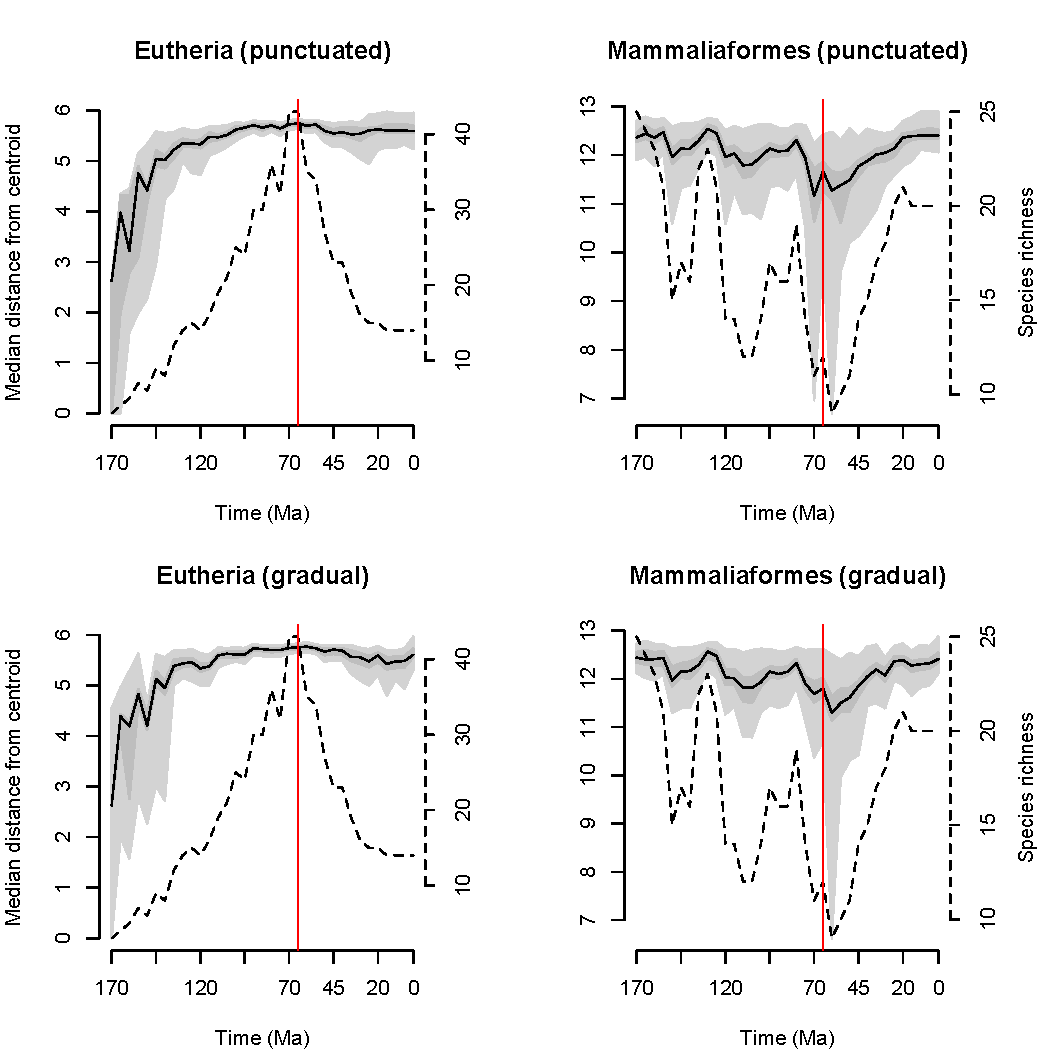
\includegraphics[keepaspectratio=true]{Figures/Main_results.pdf}
\caption{Observed variations of disparity through time among Eutherian and Mammaliaformes under punctuated or gradual evolution model. The x axis represents the time in Million of years ago (Mya). The y axis represents the disparity measured as the median distance from centroid per sub-sample. The solid black lines is the mean disparity from the bootstrapped pseudo-replicates; the confidence intervals (CI) are represent by the grey polygons (50\% CI in dark grey and 95\% CI in light grey). The dashed line represent the species richness in each sub-sample (values are reported on the right hand side of each graphs). The red vertical line represents the K-Pg boundary (66 Mya).}
\label{fig:Fig_Raw_results}
\end{figure}

\begin{figure}[!htbp]
\centering
    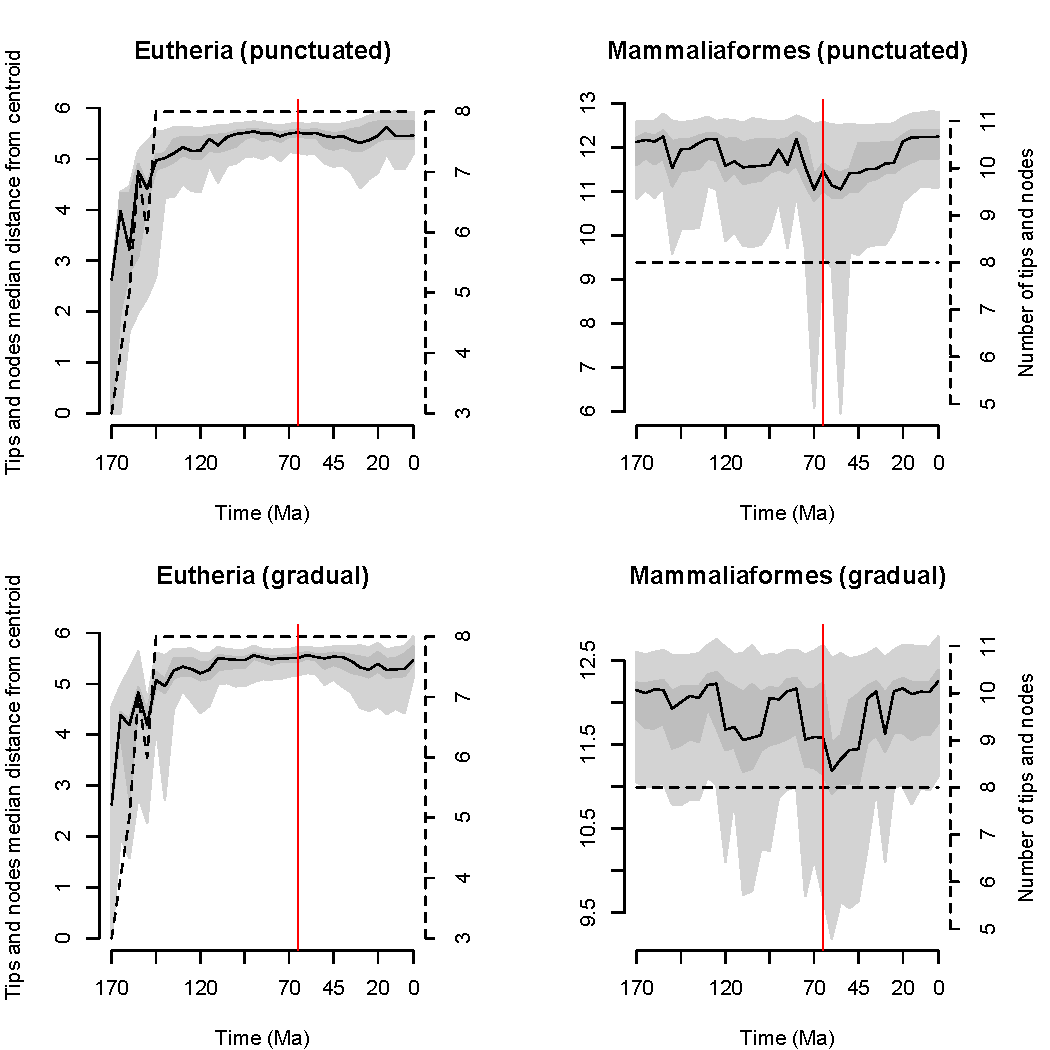
\includegraphics[keepaspectratio=true]{Figures/Main_results_rarefied.pdf}
\caption{Rarefied variations of disparity through time among Eutherian and Mammaliaformes under punctuated or gradual evolution model. The x axis represents the time in Million of years ago (Mya). The y axis represents the disparity measured as the median distance from centroid per sub-sample. The solid black lines is the mean disparity from the bootstrapped pseudo-replicates; the confidence intervals (CI) are represent by the grey polygons (50\% CI in dark grey and 95\% CI in light grey). The dashed line represent the species richness in each sub-sample (values are reported on the right hand side of each graphs). The red vertical line represents the K-Pg boundary (66 Mya).}
\label{fig:Fig_Rar_results}
\end{figure}

\begin{landscape}
\begin{table}[ht]
\caption{Permanova results of testing the effect of time on the ordinated distance matrix using euclidean distance with 1000 permutations. Data: Eutherian \citep[data from][]{beckancient2014}; Mammaliaformes, \citep[data from][]{Slater2012MEE}. Model: evolutionary model. Significant effects are highlighted in bold: one star (*) signifies a p-value between 0.05 and 0.005; two starts between 0.005 and 0.0005 and three stars $<$ 0.0005.} %Or just say three stars since it's the only results?
\label{tab:Tab_permanova}
\centering
\begin{tabular}{rrrcccccccc}
  \hline
 Data & model & terms & Df & Sum of squares & Mean sum of squares & F Model & $R^2$ & p-value & \\ 
  \hline
Eutherian     & gradual    & time      & 34  & 1825.92  & 53.703  & 1.5784 & 0.0769 & \textbf{0.0009}& \textbf{***} \\ 
              &            & residuals & 644 & 21911.65 & 34.024  &        & 0.9231 &  &\\ 
              & punctuated & time      & 34  & 1597.07  & 46.973  & 1.3693 & 0.0674 & \textbf{0.0009}& \textbf{***} \\ 
              &            & residuals & 644 & 22092.28 & 34.305  &        & 0.9326 &  &\\ 
Mammaliaformes & gradual    & time      & 34  & 6525.61  & 191.930 & 1.1660 & 0.0663 & \textbf{0.0009}& \textbf{***} \\ 
              &            & residuals & 558 & 91852.55 & 164.610 &        & 0.9337 &  &\\ 
              & punctuated & time      & 34  & 5662.25  & 166.530 & 1.0005 & 0.0574 & 0.4765 &\\ 
              &            & residuals & 558 & 92877.75 & 166.450 &        & 0.9425 &  &\\ 
   \hline
\end{tabular}
\end{table}
\end{landscape}


%TG: don't know why these tables are sent to the end of the document...
\begin{table}[ht]
\caption{Results of the \textit{post-hoc} t-tests for comparing the disparity at the last sub-sample of the Cretaceous (65 Mya) to all the sub-samples of the Cenozoic for the Eutherians \citep[data from][]{beckancient2014}. Sub-samples: reference sample (65 Million years ago; Mya) to Cenozoic sample (from 60 Mya to present). Gradual: gradual evolution; punctuated: punctuated evolution. Difference: mean sub-sample difference; Df: degrees of freedom; T: T statistic; p-value: adjusted p-value using Holm-Bonferroni correction. Significant differences are highlighted in bold: one star (*) signifies a p-value between 0.05 and 0.005; two starts between 0.005 and 0.0005 and three stars $<$ 0.0005.}
\label{tab:Tab_beck_raw}
\centering
\begin{tabular}{r|ccccl|ccccl}
  \hline
  Sub-samples & \multicolumn{5}{c|}{Gradual} & \multicolumn{5}{c}{Punctuated} \\
  (Mya) & Difference & Df & T & p.value & & Difference & Df & T & p.value &\\ 
  \hline
  65:60 & 0.06 & 76 & 1.055 & 1      & & 0.04 & 76 & 0.760 & 1      &\\ 
  65:55 & 0.05 & 75 & 0.999 & 1      & & 0.16 & 75 & 3.145 & \textbf{0.0310} & \textbf{*} \\ 
  65:50 & 0.15 & 68 & 2.412 & 0.2413 & & 0.08 & 68 & 1.403 & 1      &\\ 
  65:45 & 0.21 & 64 & 3.016 & \textbf{0.0478} & \textbf{*} & 0.18 & 64 & 2.685 & 0.1200 &\\ 
  65:40 & 0.18 & 64 & 2.579 & 0.1590 & & 0.13 & 64 & 2.173 & 0.4354 &\\ 
  65:35 & 0.23 & 60 & 2.840 & 0.0800 & $\cdotp$ & 0.21 & 60 & 2.962 & 0.0568 & $\cdotp$ \\ 
  65:30 & 0.27 & 57 & 2.927 & 0.0639 & $\cdotp$ & 0.29 & 57 & 3.810 & \textbf{0.0044} & \textbf{**} \\ 
  65:25 & 0.22 & 56 & 2.500 & 0.1999 & & 0.28 & 56 & 3.544 & \textbf{0.0104} & \textbf{*} \\ 
  65:20 & 0.16 & 56 & 1.922 & 0.7762 & & 0.25 & 56 & 3.117 & \textbf{0.0374} & \textbf{*}\\ 
  65:15 & 0.14 & 55 & 1.819 & 0.9670 & & 0.30 & 55 & 3.567 & \textbf{0.0098} & \textbf{**}\\ 
  65:10 & 0.14 & 55 & 1.843 & 0.9203 & & 0.42 & 55 & 4.540 & \textbf{0.0004} & \textbf{***} \\ 
  65:5  & 0.14 & 55 & 1.790 & 1      & & 0.30 & 55 & 3.377 & \textbf{0.0176} & \textbf{*} \\ 
  65:0  & 0.14 & 55 & 1.818 & 0.9692 & & 0.17 & 55 & 2.250 & 0.3705 \\ 
   \hline
\end{tabular}
\end{table}

\begin{table}[ht]
\caption{Results of the \textit{post-hoc} t-tests for comparing the disparity at the last sub-sample of the Cretaceous (65 Mya) to all the sub-samples of the Cenozoic for the rarefied Eutherians \citep[data from][]{beckancient2014}. Column heads explained same as given in table ~\ref{tab:Tab_beck_raw}.}
\label{tab:Tab_beck_rar}
\centering
\begin{tabular}{r|cccc|cccc}
  \hline
  Sub-samples & \multicolumn{4}{c|}{Gradual} & \multicolumn{4}{c}{Punctuated} \\
  (Mya) & Difference & Df & T & p.value & Difference & Df & T & p.value \\ 
  \hline
  65:60 & 0.04  & 76 & 0.218  & 1 & 0.01 & 76 & 0.064 & 1 \\ 
  65:55 & 0.04  & 75 & 0.213  & 1 & 0.14 & 75 & 0.797 & 1 \\ 
  65:50 & 0.11  & 68 & 0.553  & 1 & 0.04 & 68 & 0.224 & 1 \\ 
  65:45 & 0.15  & 64 & 0.716  & 1 & 0.13 & 64 & 0.600 & 1 \\ 
  65:40 & 0.11  & 64 & 0.544  & 1 & 0.07 & 64 & 0.358 & 1 \\ 
  65:35 & 0.15  & 60 & 0.627  & 1 & 0.12 & 60 & 0.572 & 1 \\ 
  65:30 & 0.15  & 57 & 0.636  & 1 & 0.17 & 57 & 0.772 & 1 \\ 
  65:25 & 0.10  & 56 & 0.423  & 1 & 0.16 & 56 & 0.697 & 1 \\ 
  65:20 & 0.03  & 56 & 0.131  & 1 & 0.13 & 56 & 0.555 & 1 \\ 
  65:15 & 0     & 55 & 0.005  & 1 & 0.16 & 55 & 0.674 & 1 \\ 
  65:10 & -0.01 & 55 & -0.034 & 1 & 0.27 & 55 & 1.129 & 1 \\ 
  65:5  & 0.01  & 55 & 0.029  & 1 & 0.15 & 55 & 0.640 & 1 \\ 
  65:0  & 0     & 55 & 0.005  & 1 & 0.02 & 55 & 0.071 & 1 \\
   \hline
\end{tabular}
\end{table}


\begin{table}[ht]
\caption{Results of the \textit{post-hoc} t-tests for comparing the disparity at the last sub-sample of the Cretaceous (65 Mya) to all the sub-samples of the Cenozoic for the Mammaliaformes \citep[data from][]{Slater2012MEE} under gradual evolution model. Raw data: data without correcting for taxonomic diversity; Rarefied data: rarefied bootstrapped data. Other column heads explained same as given in table \ref{tab:Tab_beck_raw}.}
\label{tab:Tab_slater}
\centering
\begin{tabular}{r|cccc|cccc}
  \hline
  Sub-samples & \multicolumn{4}{c|}{Raw data} & \multicolumn{4}{c}{Rarefied data} \\
  (Mya) & Difference & Df & T & p.value & Difference & Df & T & p.value \\ 
  \hline
  65:60 & 0.49  & 19 & 0.826  & 1      & 0.26  & 19 & 0.365  & 1 \\ 
  65:55 & 0.45  & 20 & 0.734  & 1      & 0.31  & 20 & 0.428  & 1 \\ 
  65:50 & 0.13  & 21 & 0.267  & 1      & 0.03  & 21 & 0.042  & 1 \\ 
  65:45 & -0.05 & 24 & -0.109 & 1      & 0.03  & 24 & 0.051  & 1 \\ 
  65:40 & -0.22 & 25 & -0.543 & 1      & -0.08 & 25 & -0.118 & 1 \\ 
  65:35 & -0.33 & 27 & -0.858 & 1      & -0.19 & 27 & -0.321 & 1 \\ 
  65:30 & -0.37 & 28 & -0.973 & 1      & -0.21 & 28 & -0.335 & 1 \\ 
  65:25 & -0.48 & 30 & -1.358 & 1      & -0.25 & 30 & -0.394 & 1 \\ 
  65:20 & -0.69 & 31 & -2.030 & 0.6625 & -0.44 & 31 & -0.711 & 1 \\ 
  65:15 & -0.76 & 30 & -2.201 & 0.4620 & -0.53 & 30 & -0.906 & 1 \\ 
  65:10 & -0.86 & 30 & -2.666 & 0.1593 & -0.66 & 30 & -1.241 & 1 \\ 
  65:5  & -0.85 & 30 & -2.668 & 0.1585 & -0.63 & 30 & -1.197 & 1 \\ 
  65:0  & -0.86 & 30 & -2.678 & 0.1548 & -0.62 & 30 & -1.133 & 1 \\ 
   \hline
\end{tabular}
\end{table}

%---------------------------------------------
%
%       DISCUSSION
%
%---------------------------------------------

\section{Discussion}
Our results show that there is a significant effect of time on changes in disparity under the assumption of gradual evolution in Mammaliaformes and Eutherians as well as under the assumption of punctuated evolution for Eutherians (table \ref{tab:Tab_permanova}).
However, regardless the taxonomic level (i.e. family \textit{vs.} genus) and regardless the evolutionary model (i.e. gradual or punctuated evolution), there is no significant difference in disparity between the latests Cretaceous sub-sample and any of the Cenozoic sub-samples (Figure \ref{fig:Fig_Rar_results}).
In fact the disparity seems to reach a plateau at the end of the Jurassic (150 Mya) for Eutherians and during the late Triassic (Norian; 220 Mya) for the Mammaliaformes and stays relatively constant after that (see Figure \ref{fig:Fig_Rar_results} and S4 @@@).
These results shows that, within the frame of our data-sets, we did not detect any short term or long term effect of the K-Pg event on mammalian disparity.
Therefore, we argue that the extinction of the many terrestrial vertebrates (namely non-avian dinosaurs) at the K-Pg boundary did not directly affected mammals evolution during the Cenozoic, or at least their morphological diversity.
% TG: just a thought: actually this is pretty intuitive. Even if the Cenozoic display the emergence of some crazy shapes (i.e. wales and bats), most of the stuff are just rats-like creatures that where apparently already well settled deep in the Jurassic.

\subsection{Global pattern of disparity} %TG: header can probably go away later on.
The observed global patterns of changes in disparity are consistent with previous studies on mammalian disparity and on disparity in metazoans in general.
The patterns of disparity seems to plateau at their maximum disparity early in their history (approximatively after 25\% and 12\% of their history in respectively Mammaliaformes and Eutherians).
In fact, this quick increase in disparity early in history is consistent with disparity patterns in metazoans \citep{Hughes20082013}.
Additionally, as showed previously, disparity display a pattern decoupled from taxonomic diversity \citep{slaterCetacean,ruta2013,hopkinsdecoupling2013}.

\subsection{Effect of the K-Pg boundary on mammalian disparity}
The results for the Mammaliaformes data-set disparity variation are consistent with the most recent studies of Mammalian disparity, showing and early peak of disparity in the Early to Middle Jurassic \citep{Close2015}.
However, our results for Eutherians differ from \cite{Grossnickle2013} that showed a significant decrease in disparity during the late Cretaceous \citep[but see][]{Wilson2012}.
These differences can be due to the different input data to calculate disparity (morphometric data in \citealt{Grossnickle2013}; and cladistic data in the present study; but see \citealt{hetherington2015cladistic}), the different method to calculate disparity through time (time bin in \citealt{Grossnickle2013}; and time slicing in the present study; see below) or the different focal morphological aspect (dental morphology in \citealt{Grossnickle2013}; and overall - including dental - morphology in the present study).
Furthermore, we found a fundamental difference with \cite{Slater2012MEE} which shows solid evidences for a change in mode of body mass evolution at the K-Pg boundary using the same data set as in this study.
We argue that this difference can be due to the number of traits used in \cite{Slater2012MEE} and the present study.
In this study we look at an aggregate of discrete traits (the 446 morphological characters) in opposition of one continuous trait \citep[body mass in][]{Slater2012MEE}.
Both variation in morphology (i.e. from cladistic data) and variation in body mass are two different and aspects of diversity and can likely be decoupled in the same way as taxonomic diversity is decoupled from disparity. 
However, we believe our results show some robustness because the same absence of signal of an eventual effect the K-Pg boundary as been found in two independent data sets \citep[i.e.][]{Slater2012MEE,beckancient2014}.
Furthermore, our results only suggest that disparity is not affected by the K-Pg boundary but they do not allow us to assess the effect of the K-Pg boundary on changes in body mass evolution. % TG: or is that useless?
%link to caveats
Besides, few caveats can be underlined.  % TG: Bleuah. When will we be able to do bullet points discussions?

%Caveats
Firstly, both our data sets are limited.
They do not represent the full known mammalian taxonomic diversity, especially during the Neogene (23--2.58 Mya) where no fossils were represented in both data sets.
However, this might not cause a serious under-sampling problem, at least in the Mammaliaformes dataset, since their diversity peaked during the late Cretaceous \citep[Campanian; 72.1--83.6 Mya; ][]{Newham201432}.
Additionally \cite{Raia2012} have shown that mammalian diversification rates declined throughout the whole Cenozoic.
In our study, these findings could suggest that an effect of the K-Pg boundary would be more likely detected during the Palaeogene when mammalian diversification rates where still high.
Also, both data sets contains cladistic data for only a few living mammals which can also have a effect of topological accuracy \citep{GuillermeCooper,MissingMammals}.
However, both original phylogenies where built using strong topological constraint to avoid such a caveat \citep{Slater2012MEE,beckancient2014}.

Secondly, the core of the debate in mammalian evolution is weather \textit{placental} mammals originated before or after the K-Pg boundary \citep{dosReis2012,O'Leary08022013,Springer09082013,O’Leary09082013,dosReis2014}.
The infraclass Placentalia can be defined as ``the least inclusive clade that includes all extant placentals'' \citep{beckancient2014}.
However, part of the dating debate might be due to the lack of clear characters that can be used to define early placental mammals \citep{bininda2012rocking,beckancient2014}. % What IS a placental mammal?
\cite{Cartmill2012} also argues that the use of higher taxa definition in general might be obsolete since ``there is only a long, geologically slow cascade of accumulating small apomorphies''.
Therefore, in this study, we made the deliberate choice to focus on the taxonomic levels (genus \textit{vs.} family) rather than on the higher clades definitions.
We argue that if a significant change in disparity occurred at the K-Pg boundary in any of such infraclass (Placentalia, Marsupialia, etc...) it would be detectable even at a higher level (i.e. changes in Placentalia correspond by definition to changes in Eutheria and Mammaliaformes).
Also, using Total Evidence tip-dated trees provides more accurate estimates of diversification times (\citealt{ronquista2012,Wood01032013,beckancient2014}; but see \citealt{Arcila2015131}) and allows the opportunity to look at changes in disparity for both living and fossil species.

%Better link. Finish by insisting: These results suggest that the extinction of non-avian dinosaurs any many other terrestrial vertebrate clades at the end of the Cretaceous did not affect mammalian evolution.
% Therefore, we argue that the extinction of the many terrestrial vertebrates (namely non-avian dinosaurs) at the K-Pg boundary did not directly affected mammals evolution during the Cenozoic, or at least their morphological diversity.
% Here we argue that there is no evidences for a release of ecological niches \citep[e.g. ``empty'' niches;][]{archibald2011extinction} or competition pressures \citep[e.g.][]{Lovergrove} in mammals after the K-Pg boundary.

\subsection{Methodology improvements for measuring disparity}
Additionally, throughout this paper, we propose several incremental changes to the classic ways to measure disparity.
This is how we believe they improve disparity through time analysis:
% TG or no need for a list?
\begin{enumerate}
    \item \textbf{Using all the axis of the cladisto-space.}
    Previous studies focusing on disparity have used various ways to select a sub-sample of the the full cladisto-space (i.e. a sub-sample of the ordinated distance matrix) arguing that the $m$ first axis of the cladisto-space usually bear most of the data-set's variance \citep[e.g][]{brusatte50,cisneros2010,prentice2011,anderson2012using,Hughes20082013,bentonmodels2014}.
    For example in \cite{Brusatte12092008} and \cite{toljagictriassic-jurassic2013}, the authors decided to select only the $m$ first dimensions that represent up to 90\% of the variance in the distance matrix.
    The cut-off value is either given arbitrary or by visually detecting a substantial break in the slop of a scree plot of the variance per axis \citep{Wills1994}.
    We argue that even if the last dimensions of the cladisto-space bears a trivial amount of variance, there is no statistical justification to exclude them.
    However, by doing so, we included dimensions of the cladisto-space with a near 0 variance and range (variance of $2\times10^{-14}$ and $1.15\times10^{-15}$ and range of $7.31\times10^{-7}$ and $3.33\times10^{-7}$ in respectively \citealt{Slater2012MEE} and \citealt{beckancient2014})
    This makes the calculation of certain disparity metrics impossible (see below).
    An alternative method to avoid these near 0 dimensional axis problem is to simply not ordinated the data and measure disparity just from the $k$ distance matrix \citep[e.g.][]{bensonfaunal2014,Close2015}.
    \item \textbf{Using the median distance from centroid as a disparity metric.}    
    As stated above (see methods section), we deliberately chose to use the median distance from centroid as a metric from measuring disparity among many other \citep[e.g.][]{Wills1994,Ciampaglio2004,thorneresetting2011,hopkinsdecoupling2013,huang2015origins}.
    Using this metric gave use several advantages upon the four classic sum and products of ranges and variance.
    First, this metric comes with no special statistical assumptions (c.f. sum and products of variance \textit{and} covariance). % TG: now not sure about the practicality of this one as mentioned in the methods part. The stats assumptions is true no mater what but I have the feeling that covariances = 0 even with PCO.
    Secondly, this metric is not affected by the last dimensions of the cladisto-space problem (see above).
    And thirdly, this metric seems less coupled with taxonomic diversity (especially for the products of ranges and variance and the sum of ranges, see supplementary figures @@@).
    \item \textbf{Using time slicing method.}
    Contra to numerous studies focusing on disparity \citep[e.g][]{cisneros2010,prentice2011,Hughes20082013,hopkinsdecoupling2013,bentonmodels2014,bensonfaunal2014}, we chose not to bin our data in time intervals but rather to look it as a continuous process.
    We argue that by doing so, we can avoid two caveats of such method: 
    \begin{enumerate}[(i)]
        \item firstly, using time intervals based on biostratigraphy is tautologic.
        In fact, such method is likely to artefactualy emphasize disparity differences between time intervals because the same time intervals are based on notable differences in fossil fauna and flora (see supplementary figures @@@ where differences in disparity through time are much more contrasted in the interval methods than in the slicing methods).
        But note that not all studies use biostratigraphy and sometimes arbitrarily time bins of equal duration are used which also fix this caveat \citep{Butler2012,hopkinsdecoupling2013,bensonfaunal2014}.
        \item secondly, in both cases (time bins based on biostratigraphy or arbitrary durations), such method does not allow to specify assumptions on the evolutionary model.
        In fact, the underlying assumption to such method is that changes in disparity occur between the time intervals in a punctuated evolutionary model fashion.
        Although directional gradual evolution has been shown to be rare, punctuated (i.e. stasis) and gradual (i.e. random walk) evolution have been shown to be both relatively common \citep{Hunt20112007,Hunt21042015}.
        Therefore, assuming that evolution is only punctual might be erroneous in some cases and for some traits.
    \end{enumerate}
    \item \textbf{Allowing to choose the evolutionary model.}
    Finaly, using the time slicing method, allows use to crudely specify the evolutionary model for changes in disparity.
    Within Eutherians, we showed both support for an effect of time on disparity under both models of evolution.
    This can reflect the complex combination between the two modes of evolution where morphology (i.e. as inferred from the cladistic data) varies stochastically through time with a mix of random walks (i.e. gradual model) for certain set of characters and stasis (i.e. punctuated model) for others.
    These results are consistent with previous findings \citep{Hunt20112007,Hunt21042015}.
    It is also encouraging to see that the distinction between the two modes of evolution can help understanding the patterns of changes in disparity at a finer scale.
    In fact, for Mammaliaformes, there is no significant effect of time on disparity under the assumption of a punctuated model of evolution but a clear effect of time when evolution is assumed to be gradual (see Table 1@@@).
    When looking at the details of this results, the same data sets shows also no significant effect of time when using the time bin method (including nodes) or when assuming that disparity evolves under an ACCTRAN model (see supplementary permanova results @@@).
    This suggests that there is an effect of time on Mammaliaformes with mix between punctuated delay evolution (DELTRAN) and gradual evolution (random walk).
    This could be interpreted as when a particular morphology (i.e. a set of particular states for cladistic characters) is observed within a clade, this particular morphology will be likely conserved through time.
    Other common but more complex models could also be implemented such as a combined stasis and random walk \citep{Hunt21042015} or models based on morphological rates rather than just the sheer branch length.
    For example, one could use a density of probability for choosing the ordinated data for either the descendant or the ancestor based on morphological clocks rather than just branch length.
\end{enumerate}
Two major caveats, however, arise from using such a method.
First, this method relies on good estimates of characters states at the nodes of the phylogeny.
Estimating discrete ancestral characters can sometimes be tricky and can lead to low scaled likelihood values supporting any states of a particular character, especially when many data are missing in the observed cladistic matrix.
However, in this particular study, we made the methodological choice of selecting only characters with a high scaled likelihood support ($> 0.95$).
Additionally, using trees containing fossil taxa also improves the ability to correctly estimate ancestral characters \citep{Poly2001,Finarelli2006,Albert2009,Slater2012MEE}.
Finally, because, this method samples every phylogenetic element (tip, node or edge) through time, disparity calculated close to the root of the tree can exhibit result with large confidence intervals (e.g. when only three phylogenetic elements are sampled see Figure S3 and S@@@).
However, it is encouraging to note that measuring disparity from time-slices is decoupled from taxonomic diversity at least after a minimal number of taxa \citep{slaterCetacean,ruta2013,hopkinsdecoupling2013}

%Conclusion
In summary, the majority attempts to solve the debate on whether placental mammals diversified after or before the K-Pg boundary is based on taxonomic diversity and shows unclear evidences on weather the K-Pg extinction event had an effect on mammalian diversification \citep{meredithimpacts2011,O'Leary08022013,dosReis2014,beckancient2014}.
Among the variety of macroevolutionary process proposed to support an effect of the K-Pg boundary on mammalian evolution, some authors proposed the release of ecological niches after the K-Pg boundary \citep[e.g.][]{archibald2011extinction,O'Leary08022013} or a release of competition pressures \citep[e.g.][]{Slater2012MEE,Lovergrove}.
In this study, however, we proposed a different approach looking at morphological diversity (i.e. disparity) through time using a continuous time sampling approach that allows use to specify assumption on the mode of evolution (i.e. punctuated or gradual).
We based our analysis on the palaeontological discoveries of the last decade showing an unprecedented and unexpected taxonomic and morphological diversity prior to the Cenozoic \citep{luo2007,Close2015}.
We found no evidences for an effect of the K-Pg boundary on changes in mammalian disparity at both the family and the genus level and under both assumption of gradual or punctual evolution.
We therefore suggest that, contra to popular believe, the extinction of many terrestrial vertebrates (namely the dominant non-avian dinosaurs) did not significantly affect the evolution of mammals throughout the Cenozoic.

%---------------------------------------------

\section{Data availability and reproducibility}
Data will be available on Dryad or Figshare.
Code for reproducing the analysis is available on GitHub (\url{ithub.com/TGuillerme/SpatioTemporal_Disparity}).

\section{Acknowledgments}
%Thanks to Graeme Lloyd, Andrew Jackson, Gavin Thomas and Sive Finlay.% for their useful comments on measuring disparity.
%Calcualtions where performed using the Lonsdale cluster maintained by the Trinity Centre for High Performance Computing and funded through grants from Science Foundation Ireland. %TG: I actually did use the cluster but only because I'm lazy and impatient. It can definitely run on a laptop (probably between one evening and one week-end running). Should I still say I used the cluster? Or will it make it sound like it's heavy calculations?

\section{Funding} % NC: Usually this is part of acknowledgments.
This work was funded by a European Commission CORDIS Seventh Framework Programme (FP7) Marie Curie CIG grant (proposal number: 321696).

 %   \citept{key} ==>>                Jones et al. (1990)
 %   \citept*{key} ==>>               Jones, Baker, and Smith (1990)
 %   \citep{key} ==>>                (Jones et al., 1990)
 %   \citepp*{key} ==>>               (Jones, Baker, and Smith, 1990)
 %   \citepp[chap. 2]{key} ==>>       (Jones et al., 1990, chap. 2)
 %   \citep[e.g.][]{key} ==>>        (e.g. Jones et al., 1990)
 %   \citepp[e.g.][p. 32]{key} ==>>   (e.g. Jones et al., p. 32)
 %   \citepauthor{key} ==>>           Jones et al.
 %   \citepauthor*{key} ==>>          Jones, Baker, and Smith
 %   \citepyear{key} ==>>             1990

\bibliographystyle{sysbio}
\bibliography{References}

% \section{supplementaries}

% \subsection{Ancestral states estimation}
% We used both the \texttt{ace} function from the R package ape v. 3.2 \citep{paradisape:2004} and the 
% \texttt{rerootingMethod} function from the R package phytools 0.4-45 \citep{phytools}. Both method perform a maximum likelihood estimation of the ancestral values and the variance of a Brownian motion process based on the re-rooting method of \citep{Yang01121995}. The two methods differ slightly in the calculation of the normalized conditional likelihoods but mainly on the way to treat missing data. We optimised the \texttt{ace} function for fast estimation by treating missing data in the matrix as an extra character (e.g. if a character has two observed tips states 0 and 1 and a third tip has missing data (NA), the ancestor of these three tips can be estimated between the three following states: 0, 1 and NA). For the \texttt{rerootingMethod}, we followed \citep{Claddis} method and treated the missing in the tips as any possible observed state (e.g. if a character has two observed tips states 0 and 1 and a third tip has missing data (NA), the third tip will be considered as multi-state (0\&1) and the ancestor of these three tips can be estimated between the two following states: 0 and 1). Both methods perform similarly but the implementation of the \texttt{ace} function has a slightly lower accuracy  but is three times faster than the one for the \texttt{rerootingMethod} function (see supplementaries).
% % NC: Some of this probably belongs in methods

% \subsubsection{Time intervals}
% We then divide our observed cladisto-spaces into sub cladisto-spaces representing the different stages of the character-space filling. For example, if at various points in time.
% %The intervals should be a compromise between the resolution and the sample size and must be "sufficiently coards that nearly all generic first and last occurenaces can be unambiguously assigned" \citep{Foote01071994}.
% Time intervals from 170Ma (Earliest Cenomanian, Late Cretaceous) to the present.
% We count all the nodes/tips present in a given time interval.
% Classic but artificially grouping data. The minimal bin size should contain at least two nodes/tips and sometime that involves having time intervals spanning accross tens of millions of years. Such long duration time intervals have no real biological meaning since it is unlikely that all of the nodes/tips present in the time interval did ever coexisted and had ever biological interactions together.

% \subsection{Diversity}
% -Diversity in living mammals
% -Diversity per interval

% \subsection{Disparity}
% -Centroid is less correlated with diversity
% -Other metrics

% \subsection{Not to be in the paper, neither in the supplementaries (methods table)}

% \begin{table}[ht]
% \caption{Comparison of Cladisto-space studies methods}
% \centering
% \begin{tabular}{cccccccc}
%   \hline
%     Date & Author      & Distance  & axis & Binning    & Disparity   & Difference & cite \\ %
%   \hline
%          & this study  & Gower     & PCO        & Time slice & centroid    & NPMANOVA?  & \\
%     2014 & Benson      &           &            & Equal bins & Wills 1994* & NPMANOVA   & \citep{bensonfaunal2014} \\
%     2014 & Brusatte    & Euclidean & PCO        &            &             &            & \citep{brusattegradual2014} \\
%     2014 & Benton      & Euclidean & PCO        & Biostrat   & Wills 1994* & NPMANOVA   & \citep{bentonmodels2014} \\
%     2013 & Hopkins     &           &            & Equal bins & Wills 1994* &            & \citep{hopkinsdecoupling2013} \\             
%     2013 & Ruta        & GED       & 10 first   & Biostrat   & Wills 1994* & NPMANOVA   & \citep{ruta2013} \\
%     2013 & Hughes      & Euclidean &            & Biostrat   & Sum of var  &            & \citep{Hughes20082013} \\
%     2013 & Toljagic    & Euclidean & 90\% var   & Biostrat   & Wills 1994* & NPMANOVA   & \citep{toljagictriassic-jurassic2013} \\
%     2012 & Brusatte    & Euclidean & 90\% var   & Biostrat   & Wills 1994* & CI overlap & \citep{brusattedinosaur2012} \\
%     2012 & Anderson    & Gower     & PCO        &            &             &            & \citep{anderson2012using} \\
%     2010 & Prentice    & Euclidean & PCO        & Biostrat   & Wills 1994* & NPMANOVA   & \citep{prentice2011} \\
%     2011 & Thorne      & Euclidean &            & Biostrat   &             & NPMANOVA   & \citep{thorneresetting2011} \\
%     2010 & Cisneros    & Euclidean & PCO        & Biostrat   & Wills 1994* & NPMANOVA   & \citep{cisneros2010} \\
%     2008 & Brusatte    & Euclidean & 90\% var   & Biostrat   & Wills 1994* & NPMANOVA   & \citep{brusatte50} \\
%     2008 & Brusatte    & Euclidean & 90\% var   & Biostrat   & Wills 1994* & NPMANOVA   & \citep{Brusatte12092008} \\
%     2005 & Wesley-Hunt &           & PCO        &            & Foote 1992  & t-test     & \citep{Wesley-Hunt2005} \\
%   \hline
% \end{tabular}
% \end{table}
% * The 4 sum and product of range and variance


\end{document}
